\section{Rastertunnelmikroskopie}

In diesem Versuch sollen mithilfe der Rastertunnelmikroskopie verschiedene Materialproben untersucht werden.
Die Technik erlaubt es, die Elektronendichte an der Oberfläche von Materialien mit atomarer Auflösung zu untersuchen.

Im Folgenden wird zunächst ein Überblick über die verwendete Technik gegeben, die in diesem Versuch benutzt wird.

\subsection{Grundlagen}

Wie bei allen Ausprägungen der Rastersondenmikroskopie wird bei der Rastertunnelmikroskopie eine Messsonde über die Oberfläche der zu untersuchenden Probe bewegt.
Bei der Rastertunnelmikroskopie wird eine Spannung wird zwischen der Oberfläche und der Messonde angelegt. Diese Spannung wird so eingestellt, dass
durch den Tunneleffekt ein messbarer Strom zwischen Probe und Sonde entsteht.
Während sich die Messsonde über die Oberfläche bewegt wird in regelmäßigen Abständen die Messgröße aufgezeichnet.

Je nach Vorzeichen der angelegten Spannung zwischen Sonde und Probe können entweder die besetzten oder die unbesetzten Zustände im Material untersucht werden.
Im Falle eines Potentialgefälles in Richtung der Spitze, können Elektronen aus der Sonde in unbesetzte Zustände in der Probe tunneln.
Im umgekehrten Fall können Elektronen aus dem Material in die Sonde gelangen und es werden somit die besetzten Zustände des Materials vermessen.

Im vereinfachten Fall einer eindimensionalen Potentialbarriere ergibt sich in erster Ordnung Störungstheorie ein exponentieller Zusammenhang zwischen dem Abstand
$d$ der Sonde von der Probe und dem Tunnelstrom $I_T$:
\begin{equation}
  I_T \propto \frac{U}{d} \exp\!\left(- Kd \sqrt{\bar{φ}}\right),
  \quad \text{\cite[(VI.1)]{lueth}}
\end{equation}
wobei $U$ die Potentialdifferenz zwischen Sonde und Probe, $\bar{φ}$ die mittlere Austrittsarbeit der Probe und der Spitze. $K$ ist eine Konstante welche abhängig vom Material zwischen Probe und Sonde ist.
Dieser Zusammenhang sorgt für die große Empfindlichkeit für Unterschiede in der Materialhöhe bzw.\ der Elektronendichte.
Große Herausforderungen sind daher eine ausreichend genaue Platzierung der Sonde und das Unterbinden von Störeinflüssen wie Erschütterungen und Vibrationen.

Die benötigte Genauigkeit zur Platzierung der Sonde wird in den meisten Rastertunnelmikroskopen durch Piezokristalle erreicht.
Die Ausdehnung dieser Kristalle lassen sich durch das Anlegen einer Spannung in der erforderlichen Präzision manipulieren.
In Piezokristallen bilden sich durch Deformation Dipole in den Kristallzellen welche ein makroskopisches elektrisches Feld zur Folge haben.
Andersrum dehnen sich die Kristalle bei anlegen eines externen elektrische Feldes aufgrund des inversen piezoelektrischen Effekts aus.
Der Piezoeffekt tritt in Kristallen auf welche keine Punktsymmetrie haben. Leitende Materialien mit freien Elektronen weisen keinen
Piezoeffekt in diesem Sinne auf.
Der optimale Piezokristall verhält sich nach einem einfachen linearen Zusammenhang:
\begin{equation}
  S = d E,
\end{equation}
wobei $S$ die relative Ausdehnung des Materials, $E$ die angelegte Spannung und $d$ der Piezokoeffizient des Materials ist.
In der Regel weisen Piezokristalle jedoch einige ungewünschte Eigenschaften auf welche Störeinfluss auf die Aufnahmen des STM haben können.
Die Ausdehnung von Piezokristallen geht nur in erster Näherung linear mit angelegter Spannung. In der Praxis können
Abweichungen vom optimalen linearen Verlauf in Höhe von bis zu \SI{25}{\percent}\cite[2.2.1]{lueth}.
Wird diese Abweichung nicht korrigiert können Fehler bei der Höhenmessung entstehen.
Außerdem treten Hystereseeffekte auf. So ist die Änderung der Ausdehnung des Kristalls bei ansteigendem externen Feld nicht die Gleiche wie bei
abfallenden Feld. Da die Spitze über dem Material Ständig die Richtung wechselt, können dadurch Fehler bei der Positionierung der Spitze entstehen.


Eine weitere Fehlerquelle ist der sogenannte thermische Drift. Die Probe kann je nach Umgebungstemperatur ihre Ausdehnung ändern. Entsprechend sollte
die Temperatur während der Messung möglichst konstant gehalten werden.

Da der Tunnelstrom von der Stärke des $E$-Feldes dominiert wird,
ist außerdem die Präparation der Sonde von großer Bedeutung.
Die Spitze muss atomare Dimensionen erreichen, um lokal $E$-Felder in der benötigten Größe erzeugen zu können.
In diesem Versuch wird Platin-Iridium-Draht gerissen, um eine möglichst geeignete Spitze zu erhalten.

Während viele aufwendigere Aufbauten im Vakuum arbeiten, wird das Rastertunnelmikroskop in diesem Versuch bei Normaldruck betrieben.
Ein Vorteil der Rastertunnelmikroskopie, gegenüber Techniken wie der Low-Energy Electron Diffraction (LEED) ist, dass die Messung im Realraum stattfindet.
Es muss keine aufwendige Fourieranalyse der Messergebnisse geschehen um eine Interpretation der Bilder zu gewinnen.


\subsection{Messmethoden}

Beim Rastertunnelmikroskop werden zwei grundsätzlich verschiedene Messmethoden verwendet:
\begin{enumerate}
  \item Messung bei konstanter Höhe
  \item Messung bei konstantem Tunnelstrom
\end{enumerate}

Die erste Methode ist empfindlich auf Höhenunterschiede der Probe, so ist es möglich, dass die Spitze die Probe berührt und zerstört wird.
Bei der Messung mit konstantem Strom wird dies vermieden.
Diese Methode ist allerdings deutlich aufwendiger, da an jedem Messpunkt zunächst die Höhe, bei dem der gewünschte Tunnelstrom erreicht wird, ermittelt werden muss.
Dies geschieht üblicherweise mit einem Regelkreis zwischen der am Piezokristall angelegten Spannung und dem gemessenen Tunnelstrom.

Um Veränderungen in der Austrittsarbeit von der Topologie der Probe unterscheiden zu können, kann zusätzlich zum Tunnelstrom bzw.\ der Höhe der Probe auch die Änderung des Tunnelstroms in Abhängigkeit der Höhe an jedem Messpunkt aufgenommen werden.

\subsection{Zu untersuchende Proben}

\paragraph{HOPG}
\enquote{Highly oriented pyrolitic graphite}~(HOPG) ist eine spezielle Variante des Graphit.
Graphit ist der Name für die Kristallform von Kohlenstoff welche in der Natur am häufigsten auftritt. Graphit und HOPG besitzt ein hexagonales Gitter  welches sich in zweidimensionalen
Schichten anordnet. Die Schichten sind zueinander versetzt. So liegen immer zwei Atome, zumindest von oben betrachtet,  übereinander. An diesen
Positionen ist die Elektronendichte, und damit auch der Tunnelstrom zur STM Spitze, am höchsten. An diesen Orten werden also die Maxima im Bild erwartet.
Abbildung~\ref{fig:hopg_structure} zeigt eine schematische Darstellung der Graphit Gitterstruktur.
\begin{figure}
  \centering
  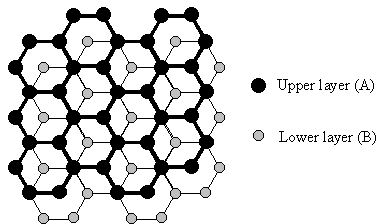
\includegraphics[width=0.6\textwidth]{images/hopg_structure.png}
  \caption{Schematische Darstellung der Gitterstruktur von Graphit.\cite{hopg_structure}}
  \label{fig:hopg_structure}
\end{figure}
In der Rastertunnelmikroskopie wird HOPG häufig zur Kalibrierung genutzt.
In diesem Versuch sollen mehrere Aufnahmen einer HOPG Probe erstellt werden,
um die Länge und Richtung der Gittervektoren des Materials zu bestimmen.
Der Literaturwert für die Gitterkonstante beträgt \SI{2.46}{\angstrom}~\cite{stm1}.

\paragraph{Gold}
Gold weist auf der Oberfläche sogenannte Stufenkanten auf. Die Höhe dieser Stufenkanten soll in diesem Versuch bestimmt werden.
Gold hat eine kubisch flächenzentrierte Gitteranordnung. Die Netzebenen der zu untersuchenden Goldprobe entsprechen den millerschen Indizes von  (111)
und somit einen Abstand in Abhängigkeit der Gitterkonstante $a=\SI{407.82}{\pico\meter}$ von $\sfrac{a}{\sqrt{3}} = \num{235.45}$\cite{stm_gold}.
Die Stufenkanten auf der Goldoberfläche sollten demnach eine Höhe von einigen vielfachen des Netzebenenabstands besitzen.
Da Gold ein guter Leiter ist, ist es schwierig die atomare Auflösung der Oberfläche zu Messen. Die Tunnelströme sind weniger lokalisiert
als bei Graphit.
